\documentclass[tikz,convert={outfile=\jobname.svg}]{standalone}

\usepackage{pgfplots}
\definecolor{line1}{RGB}{76, 44, 146}
\definecolor{line2}{RGB}{46, 133, 64}
\definecolor{line3}{RGB}{227, 28, 61}

\renewcommand{\phi}{\varphi}

\begin{document}
  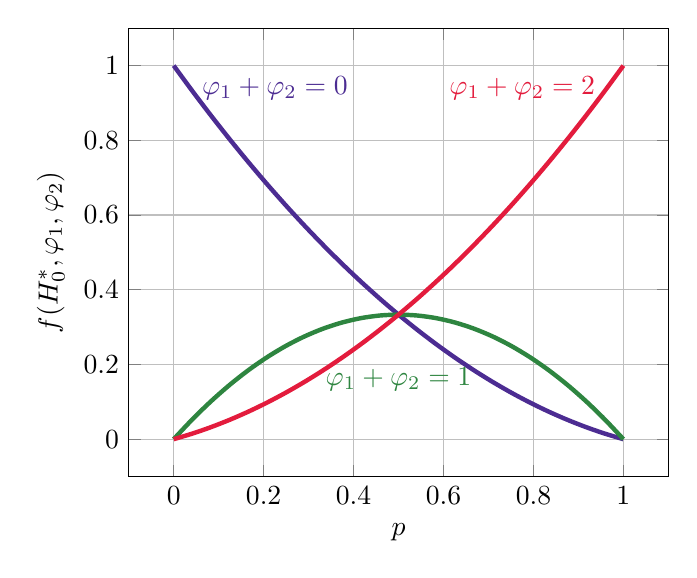
\begin{tikzpicture}
    \begin{axis}[
      xmin = -0.1, xmax = 1.1,
      ymin = -0.1, ymax = 1.1,
      xlabel = {\( p \)}, ylabel = {\( f(H_0^*, \phi_1, \phi_2) \)},
      grid = both]
      \addplot[domain = 0:1, smooth, line1, ultra thick]{(1 - x) * (1 - (2 * x / 3))}
      node[right, pos = 0.05] {\( \phi_1 + \phi_2 = 0 \)};
      \addplot[domain = 0:1, smooth, line2, ultra thick]{2 * (2 / 3) * (1 - x) *  x}
      node[below = 15, pos = 0.5] {\( \phi_1 + \phi_2 = 1 \)};
      \addplot[domain = 0:1, smooth, line3, ultra thick]{x * (1 - (2 / 3) * (1 - x))}
      node[left, pos = 0.95] {\( \phi_1 + \phi_2 = 2 \)};
    \end{axis}
  \end{tikzpicture}
\end{document}